\section{Preliminaries}
\label{sec:background}

\newcommand{\bool}[0]{\mathit{bool}}
\newcommand{\reach}[0]{\mathit{R}}
\newcommand{\ite}[3]{\mathit{if}\ {#1}\ \mathit{then}\ {#2}\ \mathit{else}\ {#3}}

%\subsection{Transition Systems and Safety Properties}
Given a state space $U$, a transition system $(I,T)$ consists of an
initial state predicate $I : U \to \bool$ and a transition step
predicate $T : U \times U \to \bool$.
We define the notion of
reachability for $(I, T)$ as the smallest predicate $\reach : U \to
\bool$ which satisfies the following formulas:
\begin{gather*}
  \forall u.~ I(u) \Rightarrow \reach(u) \\
  \forall u, u'.~ \reach(u) \land T(u, u') \Rightarrow \reach(u')
\end{gather*}
A safety property $P : U \to \bool$ is a state predicate. A safety
property $P$ holds on a transition system $(I, T)$ if it holds on all
reachable states, i.e., $\forall u.~ \reach(u) \Rightarrow P(u)$,
written as $\reach \Rightarrow P$ for short. When this is the case, we
write $(I, T)\vdash P$. To generalize the notion of transition system, especially in SMT-based model checking, it is assumed that the transition relation has the structure of a top-level conjunction. This assumption gives us a structure that we can easily manipulate. Given $T(u, u') = T_1(u, u') \land \cdots \land T_n(u, u')$ we will write $T = \bigwedge_{i=1..n}T_i$ for short.
By further abuse of notation,
$T$ is identified with the set of its top-level conjuncts. Thus, $T_i \in
T$ means that $T_i$ is a top-level conjunct of $T$, and $S
\subseteq T$ means all top-level conjuncts of $S$ are top-level
conjuncts of $T$. When a top-level conjunct $T_i$ is removed from $T$, it is written as $T \setminus \{T_i\}$. Such a transition system can easily encode our example model in Section~\ref{sec:example}, where each equation defines a conjunct within $T$ that we will denote by the variable assigned; so, $T = \{$ {\small \texttt{a1\_below, a2\_below, below, alarm, doi\_on, p1, p2}} $\}$.

The idea behind finding an IVC for a given property $P$ \cite{Ghass16} is based on inductive proof methods used in SMT-based model checking, such as K-induction and PDR \cite{NFM2012:KaGaTiWh, amla2005analysis, Een2011:PDR}. Generally, an IVC computation technique aims to determine, for any subset $S \subseteq T$, whether $P$ is provable by $S$. Then, a minimal subset that satisfies $P$ is seen as a minimal proof explanation or traceability, which is called a minimal Inductive Validity Core.

\begin{definition}{\emph{Minimal Inductive Validity Core (IVC) \cite{Ghass16}:}}
  \label{def:minimal-ivc}
  $S \subseteq T$ for $(I, T)\vdash P$ is minimal Inductive Validity Core,
  denoted by $IVC(P, S)$, iff
  $(I, S) \vdash P \wedge (\forall T_i \in S.~ (I, S\setminus\{ T_i \}) \nvdash P) $.
\end{definition}

For brevity, we use term ``IVC'' to refer to a minimal IVC. Note that, given a valid property $P$, not only $P$ always has at least one IVC from $T$, but also it may have many distinct IVCs corresponding to different proof paths. To capture the latter, the \emph{all IVCs ($AIVC$)} relation has been introduced in \cite{Ghass16, Murugesan16:renext, Ghass17Cov}.
\begin{definition}{\emph{All IVCs ($AIVC$)\cite{Murugesan16:renext, Ghass17Cov}:}}
    \label{def:allivcs}
    Given $(I, T) \vdash P$, $AIVC(P)$ is an association to all IVCs for $P$:
    $$ AIVC(P) \equiv  \{\ S~|~S \subseteq T \land  IVC(P, S)\} $$
\end{definition}

Figure~\ref{fig:ivcs} illustrates these notions by a graphical representation of IVCs for property $P = (\small{\texttt{p1 or p2}})$ in the example presented in Section~\ref{sec:example}; as shown in the picture, this property has two distinct IVCs, which means the model satisfies $P$ in two different ways:
$AIVC(P) = \{ \{ \small{ \texttt{doi\_on},
~\texttt{alarm},~\texttt{below},~\texttt{a1\_below},~\texttt{p1}\},~ 
\{ \texttt{doi\_on},~\texttt{alarm},}  \allowbreak \small{
~\texttt{below},~\texttt{a2\_below},~\texttt{p2}\} }\}$. 

%As you can see, distinct IVCs may have common elements.
%The intersection of all IVCs is called the \emph{must} set for $P$.
%And, the other elements constitute a \emph{may} set for $P$ \cite{Murugesan16:renext}:
%\begin{itemize}
%  \item   $MUST (P) = \bigcap AIVC(P)$
%  \item  $MAY(P) = (\bigcup AIVC (P)) \setminus MUST(P)$
%  \item $IRR(P) = T \setminus (\bigcup AIVC(P))$
%\end{itemize}
%\noindent Given property $P$, functions $MUST$, $MAY$, and $IRR$ partition top-level conjuncts of $T$ (model elements) into three disjoint sets \emph{must}, \emph{may}, and \emph{irrelevant}, respectively. $IRR(P)$ returns portion of the model irrelevant to the satisfaction of $P$, which in our running example is $\varnothing$.
%We have used this intuition to devise heuristics for an efficient implementation, as will be discussed in Section~\ref{sec:impl}.

\begin{figure}[t]
 \centering
  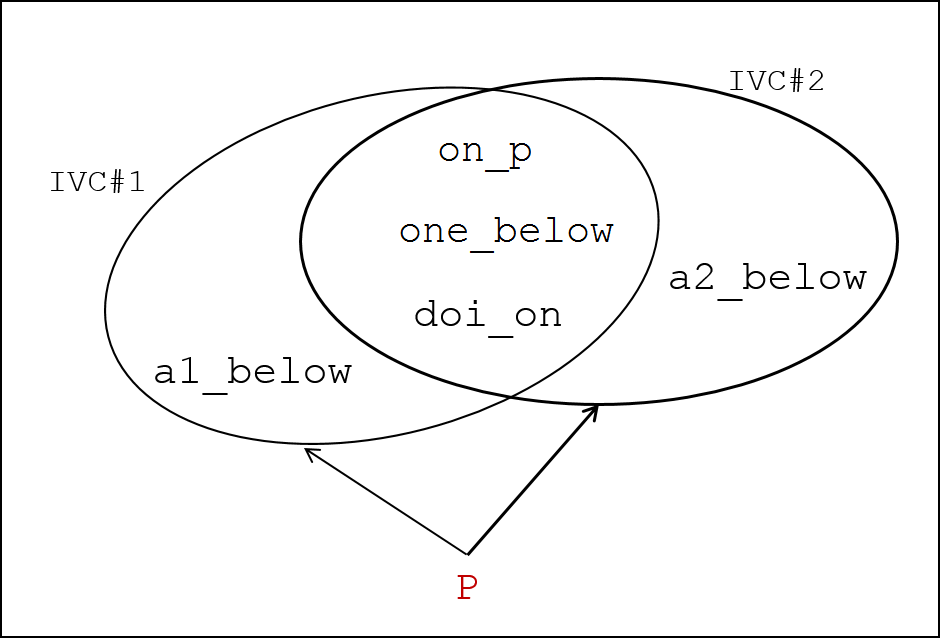
\includegraphics[width=0.9\columnwidth]{figs/ivcs.png}
  \label{fig:ivcs}
  \vspace{-0.1in}
  \caption{Graphical representation of IVCs for the model in Figure\ref{fig:asw} with  $P = (\small{\texttt{p1 or p2}})$}
\end{figure}

%\subsection{Satisfiability}
%In this subsection, we provide a brief background on satisfiability problem.
 


